Rozdział ten przedstawia szereg komercyjnie dostępnych technologii komunikacji
bliskiego zasięgu z~nakierowaniem na \gls{IoT}. Dobór właściwego rozwiązania do potrzeb
niekoniecznie jest prostą i~oczywistą decyzją~\cite{lethaby_wireless_2017, ray_edge_2019}.
Stąd też rozeznanie wśród dostępnych opcji jest niezbędną koniecznością.

Pierwszy opisany zostanie protokół ZigBee oparty o specyfikację IEEE 802.15.4. Jest to protokół
o sprawdzonej użyteczności komercyjnej będący na rynku najdłużej spośród dobranych.
Przedstawia się jego ogólną architekturę i podstawową nomenklaturę.

Thread jest stosunkowo nowym standardem na rynku. Urządzenia oparte o ten protokół stają
się coraz powszechniejsze o~czym świadczy między innymi liczba producentów wspierających
jego rozwój~\cite{noauthor_thread_nodate-1}. Nie bez znaczenia jest również postrzeganie
Thread przez branżę, upatrując w nim przyszłość rozwiązań IoT~\cite{curtis_ces_nodate-1}.

Ostatnim, tytułowym protokołem jest Bluetooth 5 wraz z jego energooszczędną odsłoną
Low Energy. Jest to najnowsze rozwiązanie na rynku z opisywanych, które ze wsparciem
organizacji Bluetooth SIG może stać się jednym z największych graczy wśród protokołów
z~przeznaczeniem do automatyki domowej.

Dla każdego z wymienionych protokołów, rozdział przedstawia krótki rys historyczny,
architekturę stosu wraz z próbą odwołania się do modelu referencyjnego OSI. Przedstawia
się parametry transmisji danych i~niezbędną nomenklaturę wprowadzoną przez standard.
Natępnie, następuje próba porównania tychże standardów. Porównywane są takie
cechy jak maksymalna dozwolona ilość węzłów, przewidywane topologie,
częstotliwości transmisji danych itd.

Bazując na zebranej wiedzy, w szczególności dotyczącej BLE i Mesh, rozdział wprowadza
czytelnika teoretycznie do dwóch przeprowadzonych doświadczeń opisywanych w kolejnym
rozdziale. Przedstawia sie obecny stan wiedzy w danym zakresie, by następnie płynnie
przejść do metodologii badań i wyników w kolejnym rozdziale.

\section{ZigBee}

ZigBee jest standardem transmisji bezprzewodowej zapewniający niskokosztową platformą
możliwą do zastosowania w elektronice użytkowej, automatyce domowej, wszelkiego rodzaju sensorach
(w~szczególności przemysłowych i~medycznych) jak również grach i~zabawkach.
Pierwsza specyfikacja opublikowana została w grudniu 2004 roku będąc ciągle aktualizowana,
z najnowszą jej wersją będącą datowaną na marzec 2017 roku~\cite{zigbee_alliance_zigbee_2017}.

Architektura ZigBee oparta została o IEEE 802.15.4. Definiuje ona fundamentalne zagadnienia:
\gls{PHY} i~\gls{MAC}. Warstwa fizyczna odpowiada za funkcjonowanie
radia, \gls{LQI}, transmisję danych i~odbiór pakietów poprzez łącze fizyczne. Definiuje dozwolone
częstotliwości działania, szerokości pasma, rodzaj modulacji i~dozwoloną przepustowość danych
wyrażonych w bitach na sekundę. Warstwa MAC odpowiada za komunikację w wyższych warstwach stosu.
Obejmuje to między innymi zarządzanie dostępem do kanałów, walidacja ramek danych, informację
zwrotną o~otrzymaniu i~przetworzeniu danych~\gls{ACK} oraz zapewnia odpowiednie
uchwyty celem umożliwienia wdrożenia mechanizmów zabezpieczeń.

\begin{figure}[!ht]
	\centering 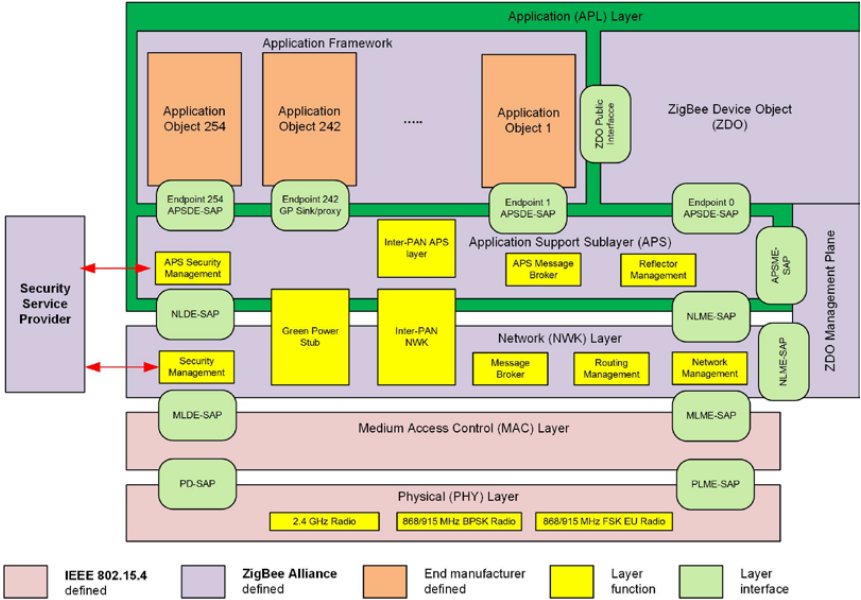
\includegraphics[width=0.99\linewidth]{zigbee_stack_architecture.png}
	\caption{Architektura stosu ZigBee. Źródło:~\cite{zigbee_alliance_zigbee_2017}}
	\label{rys:zigbee_stack_architecture}
\end{figure}

Standard wprowadza również pojęcie topologii uwzględniając tym samym sposoby,
w~jakich można zorganizować sieć poszczególnych urządzeń. Definiowane są dwie
opcje połączeń: gwiazda, peer-to-peer. Topologia gwiazdy pozwala podłączenie wielu węzłów
uwzględniając fakt, iż komunikacja odbywa się za pośrednictwem koordynatora \gls{PAN},
będący tożsamy z \gls{FFD}. W~przypadku konfiguracji rówieśniczej, urządzenia mogą 
komunikować się dodatkowo między sobą, zapewniając możliwość ustanowienia innych struktur, m.in. 
Mesh. Standard wprowadza określenie \gls{RFD}, będące najczęściej urządzeniem o~prostej funkcjonalności 
niewymagającym dużych ilości danych do funkcjonowania, o~zredukowanej potrzebie na 
zasoby sprzętowe~\cite{ieee_p80215_working_group_ieee_nodate}.

Specyfikacja ZigBee, opierając się na dokumentach IEEE 802.15.4, wykorzystuje częstotliwości
$868/915 MHz$ (w zależności od regionu Europa albo USA/Australia) oraz 2.4GHz~\cite{zigbee_alliance_zigbee_2017}.
Umożliwia tym samym transfer z przepustowością do 250~kbps~\cite{silicon_laboratories_ug10302_2021}.
Omawiany standard wprowadza swoje dodatkowe warstwy komunikacji do stosu: \gls{NWK} oraz~\gls{APL} --
Rysunek~\ref{rys:zigbee_stack_architecture}.
Warstwa aplikacji, będącą najwyższą w~hierarchi, składa się z wielu składowych. \gls{APS} odpowiada za
komunikację pomiędzy \gls{NWK} a~warstwami wyższymi. Oferuje między innymi parowanie urządzeń,
przekazywanie wiadomości, adresację, zajmuje się fragmentacją pakietów i~zapewnia niezawodny transport danych.
\gls{ZDO} w~głównej mierze odpowiada za wyszukiwanie urządzenia i~usług ZigBee~\cite{stmicroelectronics_an5506_2020, zigbee_alliance_zigbee_2017}.
Nadaje on również role urządzeniom sieci.

\begin{figure}[!ht]
	\centering 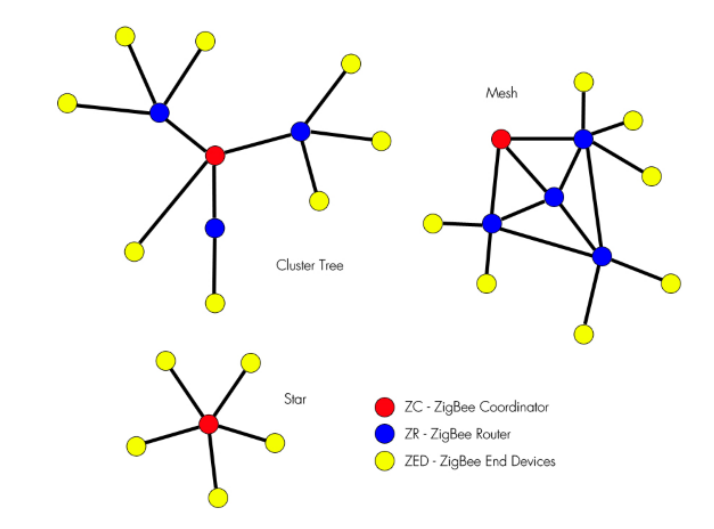
\includegraphics[width=0.618\linewidth]{zigbee_topologies_an5506.png}
	\caption{Topologie sieci ZigBee. Źródło:~\cite{stmicroelectronics_an5506_2020}}
	\label{rys:zigbee_topologies_an5506}
\end{figure}

ZigBee wprowadza trzy główne definicje ról urządzeń rejestrowanych do wewnątrz sieci:
\begin{itemize}
\item \gls{ZC} -- węzeł odpowiadający za utworzenie i~utrzymywanie scentralizowanej sieci, dobór wymaganych parametrów, dodawanie nowych węzłów.
\item \gls{ZR} -- węzeł odpowiadający za przekazywanie danych, który również może przyjąć rolę urządzenia końcowego. 
\item \gls{ZED} -- węzeł końcowy który odbiera i wysyła dane bez możliwości ich routowania.
\end{itemize}

Warstwa sieci umożliwia adaptację trzech rodzajów topologii: gwiazda, drzewo i mesh -- Rysunek~\ref{rys:zigbee_topologies_an5506}.
Typ gwiazdy kontrolowany jest przez jednego koordynatora. Topologia drzewa pozwala zastosować hierarchiczne
sposoby routingu pakietów. Typ mesh z kolei pozwala na pełną komunikację peer-to-peer między węzłami~\cite{zigbee_alliance_zigbee_2017}.
Zestawienie poszczególnych warstw z~modelem referencyjnym OSI znajduje się na Rysunku~\ref{rys:zigbee_osi_comparison_an5506}.

ZigBee umożliwia wykorzystanie następujących metod routingu. Metoda oparta o tablicę trasowania\footnote{z ang. \textit{Routing Table}}
zakłada, iż każdy z~węzłów posiada strukturę przechowującą adresy kolejnych, otaczających go węzłów. Raz wysłana wiadomość,
będzie korzystać z~tej informacji, by przesłać pakiet do miejsca docelowego. W~przypadku niepowodzenia, pierwotny węzeł otrzyma
błąd, by ewentualnie podjąć dalszą decyzję o~ponownym wyznaczeniu trasy. Standard przewiduje wysyłanie również pakietów
przy wykorzystaniu rozgłoszenia z możliwością wyboru roli danego urządzenia. Możliwy jest również multicast. Ostatnią
opcją trasowania jest metoda wiele-do-jednego (źródła)~\cite{silicon_laboratories_ug10302_2021}.

\begin{figure}[!ht]
	\centering 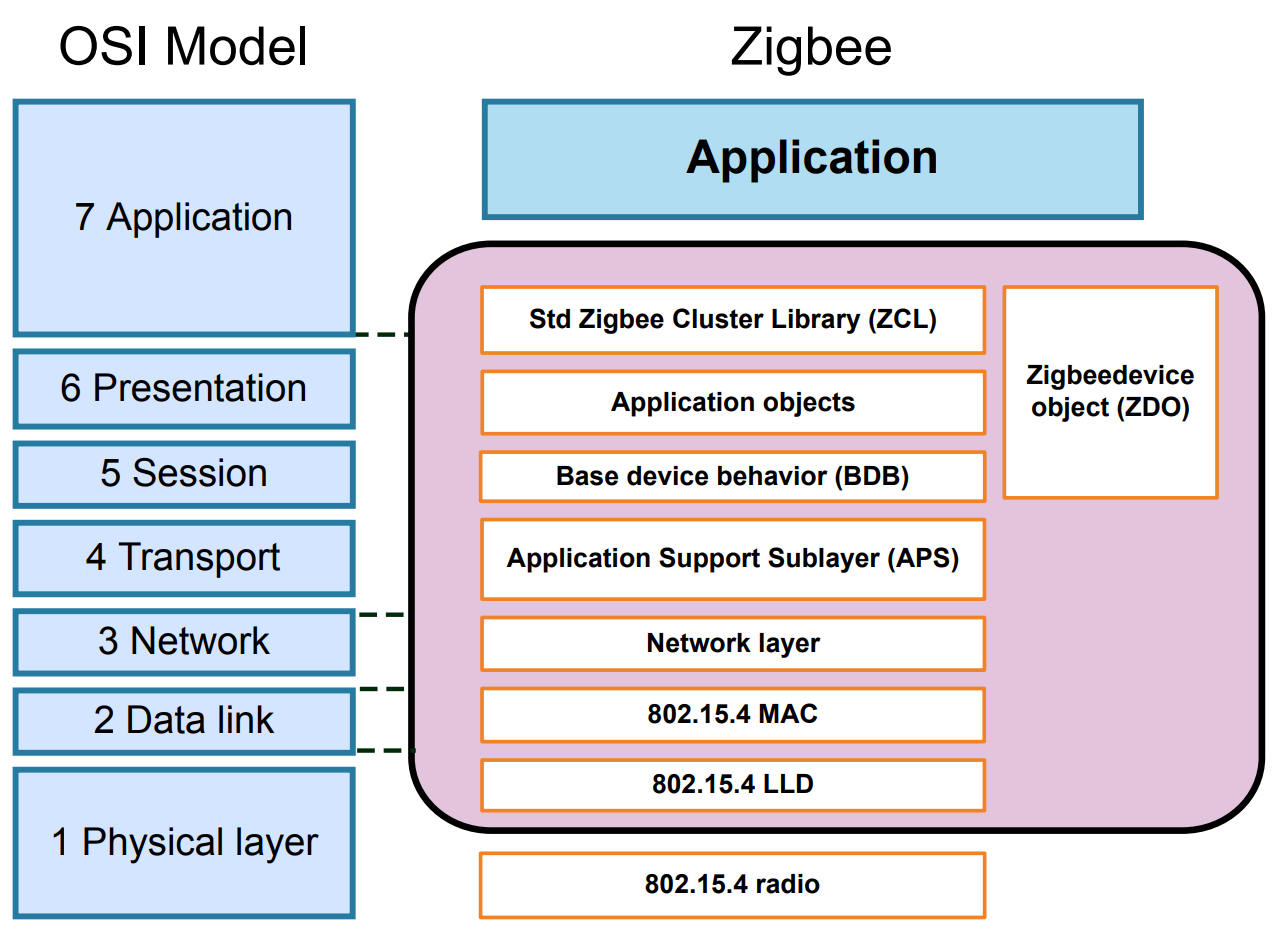
\includegraphics[width=0.618\linewidth]{zigbee_osi_comparison_an5506.png}
	\caption{Zestawienie warstw stosu ZigBee z modelem referencyjnym OSI. Źródło:~\cite{stmicroelectronics_an5506_2020}}
	\label{rys:zigbee_osi_comparison_an5506}
\end{figure}

ZigBee wprowadza termin \textit{profili}, będący kontraktem pomiędzy komunikatami wysyłanymi pomiędzy urządzeniami. Definiuje on
logiczną strukturę danych i zapewniając kompatybilność pomiędzy platformami różnych producentów. Cechą tą charakteryzują
się przede wszystkim profile publiczne zdefiniowane przez ZigBee Alliance. Poszczególni producenci mogą 
również opracować własnościowe, zamknięte struktury do tworzenia wewnętrznych sieci, gdzie kompatybilność pomiędzy
urządzeniami wielu producentów nie jest wymagana~\cite{zigbee_alliance_zigbee_2017, stmicroelectronics_an5506_2020, zigbee_alliance_zigbee_2017}.

\section{Thread}
Thread jest protokół to do zastosowań \gls{IoT} mający swe podstawy w standardzie IEEE 802.15.4.
Umożliwia on tworzenie rozwiązań o niskim zużyciu energii, przy jednoczesnej koncentracji na bezpieczeństwie opierając
adresację o powszechnie znany IPv6. Wybór IPv6 zapewnia płynną integrację z~powszechną infrastrukturą
i~Internetem włącznie. Rozwiązanie jest przez to elastyczne i~mniej podatne na starzenie się technologii.
Same natomiast produkty oparte o~Thread mogą być wdrożone na rynek szybciej dzięki powszechności
internetowych narzędzi deweloperskich. Pierwsza wersja specyfikacji została udostępniona
w 2014 roku i~pozostaje rozwijana do dziś~\cite{noauthor_thread_nodate}.

\begin{figure}[!ht]
	\centering 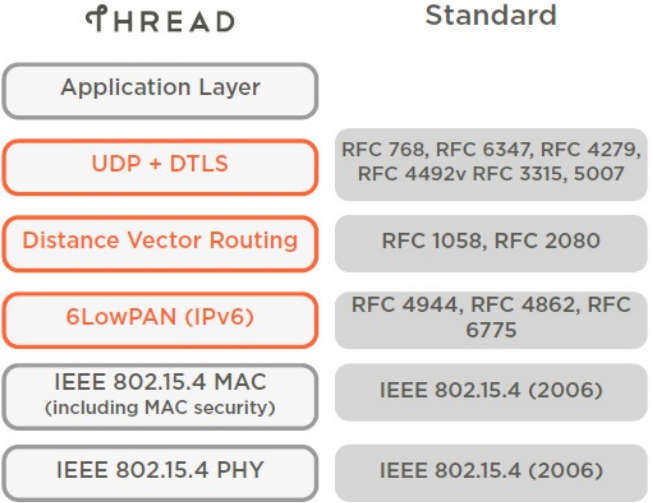
\includegraphics[width=0.618\linewidth]{thread_stack_overview_ug10311.png}
	\caption{Stos Thread i odpowiadające mu specyfikacje RFC/IEEE. Źródło:~\cite{silicon_laboratories_ug10311_2022}}
	\label{rys:thread_stack_overview_ug10311}
\end{figure}

Thread wykorzystuje standard IEEE 802.15.4. Transmisja danych odbywa się na częstotliwości $2.4GHz$ z przepustowością
do 250~kbps. Protokół jest zoptymalizowany do wykorzystywania dużej liczby węzłów wchodzących w skład sieci~\cite{silicon_laboratories_ug10311_2022}.
Celem organizacji sieci w~spójny zbiór fizycznych i~logicznych obiektów, standard wprowadza następującą nomenklaturę.
Rolą węzła typu router jest przekazywanie pakietów w sieci oraz nadzorowanie dostępu do sieci, podczas gdy radio
takiego urządzenia ciągle jest w aktywne. \gls{ED} jest urządzeniem przeważnie komunikującym się z~jednym
routerem będącym jego rodzicem, nie przekazuje pakietów dla innych sieci i~możliwością deaktywacji radia
celem ograniczenia zużycia energii. Dodatkowo, definiuje się następujące typy urządzeń:
\begin{itemize}
\item \gls{FTD} -- urządzenie posiadające ciągle włączone radio, mapujące adresację IPv6
	\begin{itemize}
	\item Router
	\item \gls{REED} -- urządzenie, które można wykorzystywać jako router
	\item \gls{FED} -- urządzenie, którego nie można wykorzystywać jako router
	\end{itemize}
\item \gls{MTD} urządzenie przekazujące komunikaty do rodzica.
	\begin{itemize}
	\item \gls{MED} -- urządzenie, którego radioodbiornik zawsze pozostaje włączony. Nie wymaga periodycznego
	pobierania wiadomości z urządzenia-rodzica
	\item \gls{SED} -- urządzenie wzbudzające radioodbiornik okazjonalnie celem pobrania wiadomości.
	\end{itemize}
\end{itemize}
Standard przewiduje dodatkowe typy jak Thread Leader, będący dynamicznie i automatycznie wybieranym węzłem
zarządzający pozostałymi Router'ami w sieci. Border Router (router brzegowy) służy za bramkę
konwertujący komunikaty przesyłane wewnątrz sieci Thread do sieci zewnętrznych takich jak Internet~\cite{noauthor_node_2022}.

\begin{figure}[!ht]
	\centering 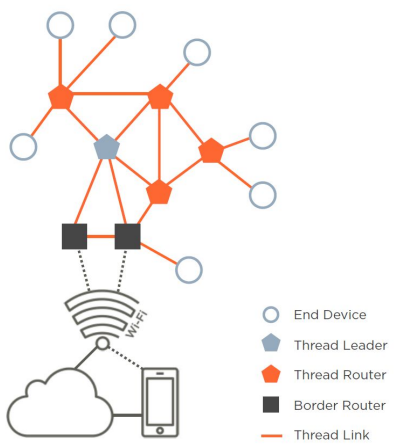
\includegraphics[width=0.464\linewidth]{thread_topology_devices_threadgroup.png}
	\caption{Podstawowa topologia sieci Thread wraz z urządzeniami. Źródło:~\cite{thread_group_thread_2020}}
	\label{rys:thread_topology_devices_threadgroup}
\end{figure}

Dane w sieci przesyłane są w oparciu o~standard \textit{6LoWPAN}\footnote{IPv6 Over Low Power Wireless Personal Networks}.
Protokół ten został zoptymalizowany w ten sposób, by wysyłać maksymalną możliwą ilość danych z użyciem jednego
pakietu celem minimalizacji fragmentacji pakietów, redukując tym samym narzut na CPU i~zużycie energii.
Thread umożliwia stosowanie również protokołów znanych z sieci opartych o model TCP/IP. Tak więc
standard ten obsługuje m.in. \gls{ICMP}, \gls{UDP}, \gls{TCP}. Topologia tym samym również zależy od ilości
węzłów typu router, tworząc albo sieć gwiazdy, albo mesh. Thread obsługuje do 32-óch routerów, gdzie każdy
z~nich może obsłużyć do 511 \gls{ED}. Routing odbywa się na zasadach znanych z~\gls{IP}
wykorzystując w tym celu protokół zbliżony do \gls{RIP}, będący zoptymalizowany do wymagań
IoT pod względem zużycia energii~\cite{silicon_laboratories_ug10311_2022}.

\begin{figure}[!ht]
	\centering 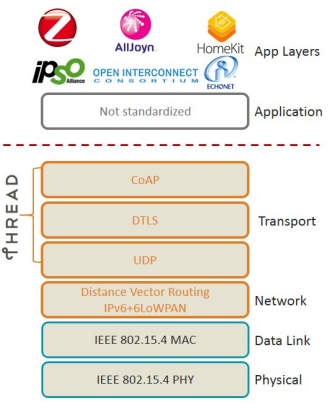
\includegraphics[width=0.618\linewidth]{thread_iso_comparison_ug10311.png}
	\caption{Thread w zestawieniu z modelem OSI. Źródło:~\cite{silicon_laboratories_ug10311_2022}}
	\label{rys:thread_iso_comparison_ug10311}
\end{figure}

Thread będący otwartym standardem może zostać wdrożony przez producenta samodzielnie bądź wybrać stos otwartoźródłowy --~Rysunek~\ref{rys:thread_iso_comparison_ug10311}.
Jednym z takich stosów jest OpenThread\footnote{\url{https://openthread.io/}} będący opracowany przez firmę Google.

Co warto dodać, Thread nie definiuje formatu danych jaki jest wysyłany pomiędzy węzłami. Innymi słowy,
warstwa aplikacji jest nieustandaryzowana~\cite{silicon_laboratories_ug10311_2022}. Obecnie trwają
prace nad opracowaniem wspólnego i~wolnościowego interfejsu. Jednym z takich projektów jest \textit{Matter}\footnote{\url{https://csa-iot.org/all-solutions/matter/}}.

\section{Bluetooth 5 - Bluetooth Low Energy}
Komunikacja bezprzewodowa $2.4GHz$ Bluetooth ma długą historię rozpoczynającą się 1998 roku~\cite{noauthor_bluetooth_nodate-1}.
Standard przeszedł wiele transformacji do postaci dzisiejszej 5.3~\cite{woolley_bluetooth_2021}. Niniejsza praca
koncentruje się na Bluetooth 5, kładąc szczególny nacisk na \gls{BLE}.

Bluetooth 5.0, ogłoszony w 2017 roku, wprowadza szereg zmian u~podstaw komunikacji radiowej. Względem poprzedzającej wersji \gls{BT},
zmodyfikowano działanie warstwy fizycznej osiągając dwukrotnie wyższe teoretyczne transfery danych, wynoszące obecnie
2 Mbps -- oznaczane jako LE 2M PHY. Zwiększono również dystans na jakim \gls{BLE} jest w stanie operować. Poprzednie
wersje BLE umożliwiały rozgłaszanie wyłącznie na 3 kanałach: 37, 37 i 39. Specyfikacja 5.0 zmieniła ten stan rzeczy
umożliwiając wykorzystywanie wszystkich kanałów, zwiększając również ilość danych które można wysłać w~pakiecie
ogłoszeniowym. Usprawniono również algorytm\footnote{\textit{adaptive frequency hopping}} doboru kanału poprawiając jakość transmisji
~\cite{woolley_bluetooth_nodate}.

Specyfikacja \gls{BT} 5.1 z roku 2019 wprowadza szereg usprawnień jak i~nową funkcjonalność. Ową funkcjonalnością jest
możliwość określenia kierunku badając różnicę w sile sygnałów z nadajników. Definiuje się dwa sposoby:
\gls{AoA} i \gls{AoD}. Pierwszy z nich polega na wysłaniu sygnału do macierzy odbiorników. W metodzie \gls{AoD}
to odbiornik odbiera sygnał z wielu nadajników mierząc przy tym fazę fali radiowej w czasie. Te funkcjonalności
mają za zadanie przygotować podwaliny pod przyszłe systemy lokalizacji w czasie rzeczywistym\footnote{RTLS - Real-Time Locating System}
oraz systemów nawigacji wewnątrz pomieszczeń\footnote{IPS - Indoor Positioning System}\cite{woolley_bluetooth_2020-1}.

\begin{figure}[!ht]
	\centering 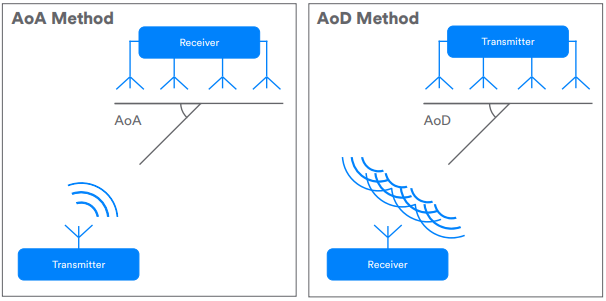
\includegraphics[width=0.618\linewidth]{bt51_aoa_aod.png}
	\caption{Lokalizowanie kierunku dla standardu Bluetooth 5.1.. Źródło:~\cite{woolley_bluetooth_2020-1}}
	\label{rys:bt51_aoa_aod}
\end{figure}

Bluetooth 5.2 z 2020 roku wprowadza nowe funkcjonalności. Ustanawia protokół \gls{EATT}, będący rozwinięciem
znanego wcześniej \gls{ATT} -- protokołu będącego u podstaw komunikacji z użyciem \gls{BLE}. Wspomniany standard
zmienia również sposób zarządzania energią. \textit{LE Power Control} umożliwia dynamiczną optymalizację
parametrów transmisji danych pomiędzy połączonymi urządzeniami poprzez monitorowanie siły sygnału. Nowa funkcjonalność
poprawia również jakość transmisji w częstotliwościach 2.4GHz, tak popularnych wśród innych protokołów
transmisji danych. Kolejnym, nowo wprowadzonym rozwiązaniem jest \textit{LE Isochronous Channels} -- kanał izochroniczny.
Umożliwiać ma ono transmisję danych do wielu urządzeń docelowych, które zostaną odebrane i~przetworzone w~tym
samym czasie. Funkcjonalność ta przewiduje główne zastosowanie w transmisji audio z użyciem BLE. Potencjalnymi
scenariuszami użycia są: współdzielenie audio z~osobami w~pobliżu, asysta słuchu, telewizja czy nawet
ogłaszanie komunikatów w~wielu językach np. na pokładzie samolotu~\cite{woolley_bluetooth_2020-2}.

Specyfikacja 5.3 z 2021 roku wprowadza m.in. usprawnienia bezpieczeństwa dla klasycznego BT BR/EDR\footnote{Basic Rate/Enhanced Data Rate}, określając
minimalną, akceptowalną długość klucza. Zapewnia również usprawnienia w~kwestii zmiany parametrów transmisji
danych -- \textit{Connection Subrating}. Zmniejsza ono opóźnienie występujące podczas zmiany wartości parametrów
zapewniając lepsze doświadczenia z~użytkowania oraz zwiększając żywotność rozwiązań zasilanych 
bateryjnie~\cite{woolley_bluetooth_2021}.

\begin{figure}[!ht]
	\centering 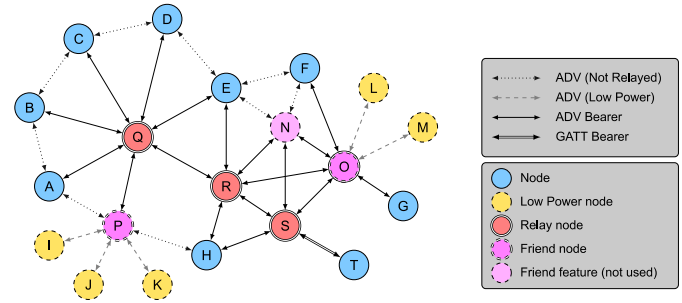
\includegraphics[width=0.618\linewidth]{mesh_topology_mesh_profile.png}
	\caption{Przykładowa topologia BT Mesh z uwzględnieniem rodzajów węzłów. Źródło:~\cite{mesh_working_group_mesh_2019}}
	\label{rys:mesh_topology_mesh_profile}
\end{figure}

Kolejnym \textit{świeżym} elementem w stosie BT to Bluetooth Mesh formanie wprowadzony
w~2017 roku. Jest to sieć wiele-do-wielu oparta o stos Bluetooth Low Energy
rozszerzając jego możliwości. Architektura warstw Mesh wygląda następująco~\cite{mesh_working_group_mesh_2019}:
\begin{itemize}
\item Warstwa modelu (\textit{Model Layer}) -- standaryzuje rodzaje operacji i~wymienianych wiadomości dla zwyczajowych przypadków użycia
\item Warstwa podstawowa modelu (\textit{Foundation Model Layer}) -- określa stany, wiadomości i~modele niezbędne do konfiguracji i~zarządzania siecią
\item Warstwa dostępu (\textit{Access Layer}) -- definiuje format danych, kontroluje szyfrowanie wiadomości, sprawdza poprawność wiadomości
pod kątem przekierowania ich do wyższych warstw
\item Górna warstwa transportowa (\textit{Upper Transport Layer})
\item Dolna warstwa transportowa (\textit{Lower Transport Layer})
\item Warstwa sieci (\textit{Network Layer})
\item Warstwa elementu nośnego/okaziciela (\textit{Bearer Layer}) -- definiuje sposób jak wiadomości są wysyłane pomiędzy węzłami
\item Specyfikacja Źródłowa BLE (\textit{Bluetooth Low Energy Core Specification}) -- stos BLE opisany zgodnie ze specyfikacją
\end{itemize}

Specyfikacja źródłowa BLE definiuje niższe warstwy wykorzystywane przez Mesh. Stanowią one analogiczną podstawę,
co IEEE 802.15.4 dla protokołów ZigBee czy Thread. Poszczególnym protokołom składowym można przypisać analogiczne
warstwy modelu referencyjnego OSI, co zostało ukazane na Rysunku~\ref{rys:agregacja_protokolow_ble}.

\begin{figure}[!ht]
	\centering 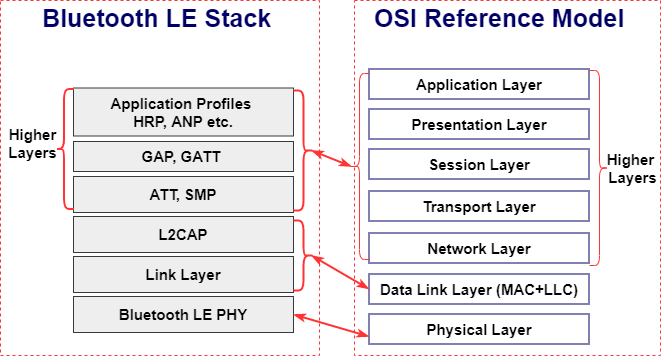
\includegraphics[width=0.618\linewidth]{mathworks_iso_osi_ble_stack.png} 
	\caption{Zestawienie stosu BLE i modelu ISO OSI. Źródło: \cite{noauthor_bluetooth_nodate}}
	\label{rys:agregacja_protokolow_ble}
\end{figure}


Węzłem określane jest urządzenie fizyczne będące zarejestrowane wewnątrz sieci Mesh. Proces, podczas którego 
następuje owa rejestracja nazywa się aprowizacją (z ang. \textit{Provisioning}). Polega on na wygenerowaniu
i~wymianie kluczy bezpieczeństwa. Szyfrowanie jest domyślne i stanowi podstawę dla konfiguracji sieci,
z której nie można zrezygnować. Pojedynczy węzeł może zawierać wiele elementów,
a te z kolei mogą zwierać wiele modeli. Elementem będzie więc niezależna składowa, która może być kontrolowana
przez dane urządzenie włączone do sieci. Model definiuje natomiast format przetwarzanych wiadomości, stany w których
węzeł może się znajdować ustalając jego zachowanie i~cechy~\cite{woolley_bluetooth_2020, st_an5292_2021}.

Węzły mogą mieć następujące dodatkowe specjalne cechy będące fundamentem dla stworzenia właściwej topologii~\cite{woolley_bluetooth_2020, st_an5292_2021}:
\begin{itemize}
\item węzeł przekaźnikowy (\textit{Relay}) -- węzeł który przekazuje dane dalej wgłąb sieci zgodnie z~algorytmem routingu do określonego momentu \gls{TTL}
\item węzeł pośredniczący (\textit{Proxy}) -- węzeł służący za bramkę, umożliwiający dostęp do sieci z~urządzenia BLE. Zrealizowane jest to poprzez
udostępnienie właściwej usługi BLE (interfejs GATT).
\item para węzłów wykorzystywanych w~których jeden z nich jest ograniczony sposobem zasilania:
	\begin{itemize}
	\item \gls{LPN} -- węzeł ograniczony zasobami sprzętowymi w tym zasilaniem, mający przeważnie za zadanie działać jak najdłużej na zasilaniu bateryjnym
	\item \textit{Friend Node} -- węzeł będący najczęściej pod stałym zasilaniem, działający w~tandemie z~\gls{LPN}, przechowując jego wiadomości
	i~oferując te dane pozostałym węzłom w sieci
	\end{itemize}
\end{itemize}

Routing w BLE Mesh oparty jest o~algorytm \textit{zalewania} (z ang. \textit{Flooding}). W~metodzie tej każda wiadomość przekazywana
jest do otaczających go węzłów wykluczając węzeł źródła danych. \gls{TTL} jest również zdefiniowany o~ilość przeskoków (z ang. \textit{hops}),
które wiadomość musi pokonać nim powinna zostać uznana za martwą.

\section{Porównanie przedstawionych standardów} 
Opisane w~poprzednich podrozdziałach protokoły i~trudność w doborze właściwego rozwiązania
do własnych zastosowań jest czymś naturalnym z czym musi zmierzyć się inżynier wraz z~zespołem
projektowym, by wybrać to \textit{najlepsze}. Poszczególne standardy komunikacji bliskiego
zasięgu leżą również w kręgu zainteresowań naukowców badając doświadczalnie ich parametry
i~zestawiając do przystępnej formy~\cite{lethaby_wireless_2017, ray_edge_2019}.

Istnieje szereg badań zestawiające wymienione wcześniej, aczkolwiek nie ograniczając się wyłącznie
do nich, protokoły~\cite{rzepecki_iotsp_2019,ray_edge_2019,noauthor_an1142_nodate,georgakakis_analysis_2011}.
Badania te wybierają parametry urządzeń i~sieci w postaci czasu oczekiwania\footnote{z ang. \textit{latency}} na przesyłane wiadomości
w~zależności od dobranego rozmiaru pakietu czy ilości węzłów, konsumpcji energii, \gls{PER}, \gls{BER},
przepustowość i~inne parametry sieci.

\begin{figure}[!ht]
	\centering 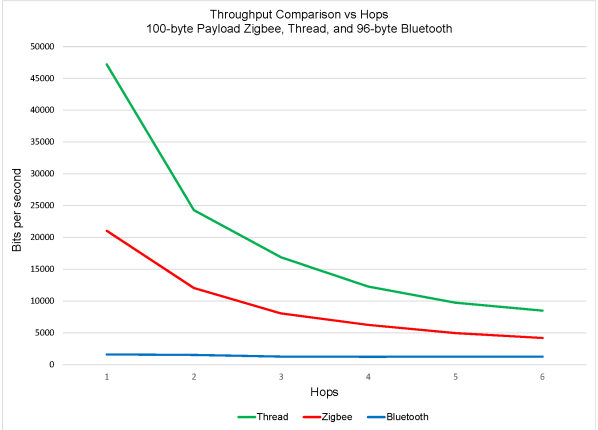
\includegraphics[width=0.618\linewidth]{throughput_vs_hops_an1142.png} 
	\caption{Porównanie przepustowości w zależności od ilości przeskoków 100-bajtowej (96-baj dla BT) pakietu podczas transmisji. Źródło: \cite{noauthor_an1142_nodate}}
	\label{rys:throughput_vs_hops_an1142}
\end{figure}

Badanie przeprowadzone przez firmę~\textit{Silicon Labs} bada i porównuje przepustowość i opóźnienie
wymienionych rodzajów sieci~\cite{noauthor_an1142_nodate}. Rysunek~\ref{rys:throughput_vs_hops_an1142}
prezentuje badanie w którym badano maksymalną przepustowość ZigBee, Thread i~BT MEsh 
w~zależności od ilości \textit{hopów}. Wykres prezentuje rezultaty testów przesyłu ~100-bajtowej wiadomości.
Dla protokołów opartych o IEEE 801.15.4 uwidacznia się wykładniczy spadek przepustowości osiągając
maksimum w komunikacji peer-to-peer, z przewagą dla Thread. Bluetooth Mesh prezentuje
stałe wartości przesyłu wiadomości. Autorzy zaznaczają, że przy tej wielkości wiadomości każdy protokół
fragmentuje ją do wielu pakietów.

\begin{figure}[!ht]
	\centering 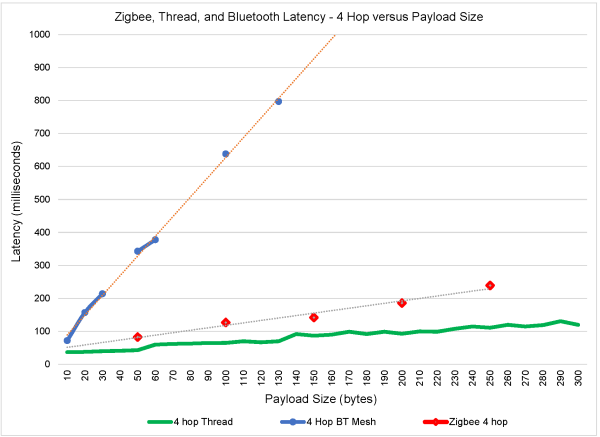
\includegraphics[width=0.618\linewidth]{latency_vs_payload_an1142.png} 
	\caption{Porównanie opóźnienia w zależności od wielkości pakietu dla 4-węzłowej sieci różnych standardów komunikacji. Źródło: \cite{noauthor_an1142_nodate}}
	\label{rys:latency_vs_payload_an1142}
\end{figure}

Inne badanie prezentuje opóźnienia występujące w sieci składających się z~4~węzłów w zależności od wielkości
wiadomości -- Rysunek~\ref{rys:latency_vs_payload_an1142}. Uwidacznia się \textit{oczywisty}
wzrost tej proporcji wraz ze większą ilością wysyłanych bajtów. Różny jest natomiast przyrost. Szczególnie wyróżnia się
tutaj Bluetooth Mesh. Ze względu na swój mechanizm routing'u\footnote{przypomnienie - flooding mechanism}
i~architekturze stosu, każda wiadomość powyżej 12 bajtów ulega segmentacji. W połączeniu z~mechanizmem routowania
sieć ulega zapchaniu powodując \textit{duży ruch} w~sieci obniżając jej możliwości transmisji. Jest to oczekiwane 
zachowanie biorąc pod uwagę architekturę stosu, który udostępniając odpowiednie usługi i~usiłuje minimalizować
ilość wysyłanych danych ograniczając się najczęściej do jednej ramki.%~\cite{noauthor_an1142_nodate,noauthor_an1137_nodate,noauthor_developing_nodate}.

\begin{figure}[!ht]
	\centering 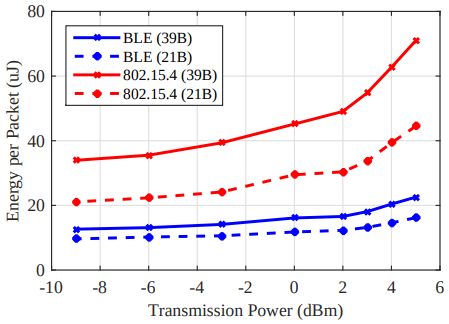
\includegraphics[width=0.618\linewidth]{energy_per_packet_dbm_10.4108.png} 
	\caption{Zależność konsumpcji energii od mocy transmisji danych w zależności od wielkości pakietu i~rodzaju protokołu. Źródło: \cite{fafoutis_ble_2016}}
	\label{rys:energy_per_packet_dbm_10.4108}
\end{figure}

Badacze analizowali również zużycie energii przez \gls{BLE} i~standard IEEE 802.15.4 z użyciem chipu
firmy \textit{Texas Instruments} -- CC2650~\cite{fafoutis_ble_2016}. Autorzy sprawdzali zależność, w~której
mierzono ilość energii niezbędnej do transmisji wiadomości o rozmiarach 21 i 39 bajtów na wysokości warstwy PHY przy
stałym napięciu zasilania 3.3V. Protokół BLE wymaga niemal dwa razy mniej energii do transmisji wiadomości
niż konkurencyjny protokół. Wraz ze wzrostem mocy nadawanego sygnału, ta proporcja staje się coraz korzystniejsza
z energetycznego punktu widzenia dla Bluetooth'a -- Rysunek~\ref{rys:energy_per_packet_dbm_10.4108}.

Protokoły również można porównać statycznie na podstawie dostępnej literatury, a przede wszystkim
publicznie dostępnych specyfikacji standardów. Rezultaty takiej analizy obserwuje się w~tabeli~\ref{tab:protokoly_zestawienie}.

\begin{table}[!ht]
\centering
	\begin{tabular}{p{2.5cm}|m{3.5cm}|m{3.5cm}|m{3.5cm}}
	Cecha porównywana & Bluetooth Mesh & Thread & ZigBee\\\hline
	Częstotliwość & 2.4GHz & 2.4GHz & 2.4GHz, 868/915MHz\\\hline
	Przepustowość & do 2Mbps & do 250 kbps & do 250 kbps\\\hline
	Max. ilość węzłów & 32767 przy max. 126 [0x7f-1] przeskokach\cite{mesh_working_group_mesh_2019} & 16352 (max. 32 routery, do 511 urządzeń końcowych/router)\cite{noauthor_node_2022} & ~64000\\\hline
	Topologia & Mesh (flooding) & Mesh & Mesh, drzewo, gwiazda\\\hline
	\end{tabular}
\caption{\label{tab:protokoly_zestawienie}Zestawienie protokołów Bluetooth Mesh, Thread, ZigBee}
\end{table}
